\title{pyGLAS version 1 documentation}
\author{
        Naushad AL Velgy \\
        Prof Philip C Biggin \\
                Department of Biochemistry\\
        University of Oxford \\
    }
\date{\today}

\documentclass[12pt]{article}
\usepackage{listings}
\usepackage[most]{tcolorbox}
\usepackage{inconsolata}
\usepackage{graphicx}
\usepackage{float}
\usepackage{wrapfig}
\usepackage{lscape}

\newtcblisting[auto counter]{sexylisting}[2][]{sharp corners, 
	fonttitle=\bfseries, colframe=gray, listing only, 
	listing options={basicstyle=\ttfamily,language=java}, 
	title=Listing \thetcbcounter: #2, #1}


\begin{document}
\maketitle

\begin{figure}[!h]
	\centering
	\includegraphics[scale=0.2]{pyGLASLogov1.png}
	\caption{pyGLAS logo}
\end{figure}

\begin{abstract}
Here we present pyGLAS, a software designed to calculate the GPCR Likeness Assessment Score (GLAS) of a GPCR. We make use of common Python packages, such as MDAnalysis, for fast calculation of specific contacts found in  crystallographically determined structures of GPCRs. pyGLAS allows for calculation of GLAS for both static snapshots (aiding in modelling of GPCRs using modelling software), or for trajectories generated from molecular dynamics (to assess the stability of GPCRs in different environments).
\end{abstract}

\newpage

\section{Introduction}
GPCRs (G Protein Coupled Receptors) are cell surface receptors responsible for transmitting signals across the membrane, from the extracellular matrix to the intracellular milieu. As such, they mediate a variety of processes, including nociception\cite{Fenalti2014}. So important are these receptors that approximately 50\% of all drugs in the market target GPCRs\cite{Cvicek2016}.

In order to better understand the nature of GPCRs, it is important to correctly model the canonical 7 transmembrane architecture, as well as the orientation of residues in critical structural motifs. Software packages, such as Modeller\cite{Sali1993} and Medeller\cite{Ebejer2013}, are commonly used to create homology models of GPCRs prior to more extensive studies into receptor-ligand interactions, allosteric modulation, free energy calculations, activation mechanism, among others.

However, excellent though these may be, Modeller and other software packages yield generic scoring functions, such as the DOPE score\cite{Shen2006}, which attempt to distinguish good models among those generated. Further steps can be taken by evaluating models using the QMEAN server\cite{Benkert2008}; however, as with the DOPE, this score is somewhat generic. It may be important, therefore, to include in our studies of GPCRs a score that is specific to the canonical structure of receptors, and that can be used to better qualify good models from poor ones.

A thorough analysis of structures deposited in the Protein Data Bank, in 2013, yielded a list of 24 interhelical contacts that are present in all activity states\cite{Venkatakrishnan2013}. A later revision of structures, in 2016, reinforced the presence of these in crystal structures where receptors existed in active states (i.e. bound to G proteins/$\beta$-arrestins), as well as in receptors in an inactive state (i.e. incapable of intracellular binding)\cite{Cvicek2016}. 

These were later termed CHICOs, or Conserved Inter Helical COntacts\cite{Cvicek2016}. The presence of these contacts was first exploited by Heifetz and colleagues\cite{Heifetz2013} in exploring agonist binding to the human Orexin-1 and Orexin-2 receptors, where the scoring variable GLAS (GPCR Likeness Assessment Score) was first introduced.

Here we introduce the first (to our knowledge) open source script to calculate the variable GLAS. We termed it pyGLAS, as it is written, and exploits well known libraries in the Python programming language. These include MDAnalysis\cite{Michauld-Agrawal2011}, Biopython\cite{Cock2009}, Numpy[12], Pandas\cite{McKinney2010} and GGPlot.

\section{Input}

\begin{wrapfigure}{l}{5cm}
	\centering
	\includegraphics[scale=0.2]{pyGLAS_input.png}
	\caption{Sample pyGLAS input. The first column refers to the pair number and the remaining column refer to the corresponding residues. Please consult [Cvicek] for details.}
\end{wrapfigure}

pyGLAS takes the following input:

\begin{itemize}
	\item A topology file (in the PDB or GRO formats; compulsory). Input using the "-r" flag.
	\item The type of output required, triggered by the "$--$format" flag. The default output is "short"; see \emph{Output type} for more on this.
	\item A trajectory file (in the XTC format; optional). Input using the "-x" flag.
	\item An option to provide a list of CHICOs and NACHOs using the "$--$chicos" and/or "$--$nachos" flags, respectively. Refer to Figure 2 for an example input CHICOs file. Please be aware that, if neither flag is triggered, pyGLAS will attempt to find the CHICOs and the NACHOs from the input file. This is done using the output from the GPCR database (reference). See Appendix 1 for more on this.
	\item Alternatively, "$--$no\_chicos"  stops pyGLAS from calculating and outputting the CHICOs. "$--$no\_nachos" is the same for the NACHOs.
\end{itemize}

\section{Output type}
pyGLAS was designed with one philosophy in mind: simplicity of output. As such, there are three output types that can be specified using the '$--$format' flag.

\subsection{"plain"}
The "plain" output was created with the goal of being used with Modeller. It will produce a text file with the GLAS of the protein and exit. The output filename is based on the input filename, such that, if your input filename is "Receptor.pdb", the output will be "Receptor.txt".

If the GLAS of "Receptor.pdb" is 19, 

\begin{sexylisting}{Some Bash}
	$ cat Receptor.txt
\end{sexylisting}

will output the number 19 to the terminal.

A quick for loop using all generated models can then be used to compare GPCR Likeness Assessment Scores. For example, in a directory with the Modeller output:

\begin{sexylisting}{Sample Bash loop for GLAS comparison}
	$ for f in *.pdb; echo $f "\t" \
	$(cat $(basename $f '.pdb').txt) \
	>> GLAS_comparison.tsv
\end{sexylisting}

The file "GLAS\_comparison.txt" should now have a list of all models generated and their respective GLAS, separated by a tab.

\subsection{"short"}
This is the default output. There are 2 streams of output based on whether a trajectory is part of the input.

\subsubsection{"short"; No Trajectory}
If the input is a single topology, pyGLAS will calculate 2 scores: the GLAS, based on the aforementioned CHICOs, and the SAS, based on the NACHOs (see Introduction). pyGLAS will output 2 files based on the input receptor filename: "filename\_GLAS.short" and "filename\_SAS.short". Figure 3 shows the output for a receptor with a GLAS of 19.

Note that this output format does not support trajectories (please see "short" and "long" for trajectory based output).

\begin{figure}[!ht]
	\centering
	\includegraphics[scale = 0.65]{pyGLAS_shortOutput.png}
	\caption{Sample pyGLAS output. The relevant sources can be found in pyGLAS/Documentation/references.txt.}
\end{figure}

\begin{figure}[h!]
	\centering
	\includegraphics[scale=0.5]{Receptor_GPCRDB_GLAS_overTime.png}
	\caption{Variation of GLAS over simulation frame. Note that pyGLAS defines the vertical axis to be between one point below lowest GLAS and 24 (so, if the lowest GLAS is 19, the vertical axis will range from 18 to 24). All plots generated by pyGLAS are saved as SVG files.}
\end{figure}

\begin{figure}[!ht]
	\centering
	\includegraphics[scale=0.8]{Receptor_GPCRDB_GLAS_long.png}
	\caption{Sample pyGLAS input. The first column refers to the pair number and the remaining column refer to the corresponding residues. Please consult [Cvicek] for details.}
\end{figure}

\subsubsection{"short': Trajectory}
If the input includes trajectory data, the output will consist of 2 plots: "filename\_GLAS\_overTime.svg" and "filename\_SAS\_overTime.svg" (see Figure 4 for an example of the former). These will track the change in the GLAS and SAS over the trajectory, and are stored in svg files (which can be viewed using software packages such as Inkscape, on Linux platforms, or Gapplin, on Mac platforms).

\subsection{"long"}
Triggering the "--format long" flag will change the output. Again, 2 streams of output will be generated based on whether trajectory data is present.

\subsubsection{"long": No Trajectory}
This output is similar to the "short" output (see FIgure 5). However, it will also write to the output files the minimum distances between the residue pairs (in Angstrom).

\subsubsection{"long": Trajectory}
Using the python library ggplot, pyGLAS will output the same graphs produced using the "short" option, and will additionally plot all minimum distances between residue pairs over time. This consists of a 4x6 canvas for GLAS residue pairs, and a 3x5 canvas for the SAS residue pairs.

\section{Test cases}
There are several directories provided with the github download: Documentation (where we are), scripts (where pyGLAS is), examples/Single\_Topology, examples/1\_Trajectory, examples/Modeller, examples/Test\_Cases and examples/High\_Temp. The latter is divided into 400K and 500K.

Each example directory has an iPython Notebook (now Jupyter Notebook) file that serves as a tutorial for using that specific branch of pyGLAS, and how each flag works.

\newpage

\bibliographystyle{acm}
\bibliography{/Users/naushadvelgy/Documents/References/pyGLAS}
\end{document}